% ─────────────────────────────────────────────────────────────────────────────
This chapter describes the methodology used to build and evaluate the BookForMe
platform, covering dataset construction, model training and selection, end-to-end
agent evaluation, and non-functional benchmark results.

% ─────────────────────────────────────────────────────────────────────────────
\section{Dataset Construction}
\label{sec:results-dataset}

\subsection{Data Collection}

\begin{description}
  \item[Real Vendor Conversations]
        With informed consent, we collected WhatsApp booking conversation logs from
        five futsal and padel court operators in Karachi (DHA, Gulshan, Clifton areas).
        Each message was assigned an intent label and relevant slot annotations.
        This source provided approximately 120 utterances covering realistic
        vocabulary and code-switching patterns.

  \item[Manual Annotation]
        Team members wrote and annotated booking queries in both English and Roman Urdu,
        targeting underrepresented intent classes (\texttt{transaction\_confirm},
        \texttt{unknown}).  This contributed approximately 180 utterances.

  \item[LLM-Driven Synthetic Augmentation]
        Following SynthDST~\cite{he2024} and An et al.~\cite{an2022}, we used       Claude Sonnet 4.5 to generate paraphrases of existing utterances in both languages,
        and to synthesise entirely new dialogues for rare classes.  Augmentation
        parameters included: back-translation (English $\to$ Urdu $\to$ English),
        lexical substitution (synonymous time expressions), and phonetic Roman Urdu
        rewriting (\textit{kal} $\to$ \textit{kull}, \textit{raat} $\to$
        \textit{raat ko}, etc.).  This contributed approximately 360 utterances.
\end{description}

\subsection{Dataset Statistics}

The full corpus comprises \textbf{694 annotated utterances} across five intent
classes. Table~\ref{tab:data-dist} shows the intent distribution over the complete
dataset (before train-only augmentation).

\begin{table}[H]
\centering
\caption{Intent distribution in the full BookForMe bilingual corpus (694 samples).}
\label{tab:data-dist}
\begin{tabularx}{0.7\textwidth}{Xrr}
\toprule
\textbf{Intent Class} & \textbf{Count} & \textbf{\% of Total} \\
\midrule
\texttt{inquiry}              & 277 & 39.9\% \\
\texttt{info}                 & 171 & 24.6\% \\
\texttt{transaction\_confirm} & 147 & 21.2\% \\
\texttt{unknown}              &  62 &  8.9\% \\
\texttt{greeting}             &  37 &  5.3\% \\
\hline
\textbf{Total}                & \textbf{694} & \textbf{100\%} \\
\bottomrule
\end{tabularx}
\end{table}

\noindent \texttt{inquiry}: user asking to check or book a slot.
\texttt{info}: user asking about price, amenities, or availability in general.
\texttt{transaction\_confirm}: user confirming a payment or referencing a transaction.
\texttt{unknown}: out-of-scope or unintelligible messages.
\texttt{greeting}: salutations and conversation openers (e.g., ``hi'', ``salam'').

The dataset was split into \textbf{485} training, \textbf{104} validation, and
\textbf{105} test samples (all original, stratified; minimum 5 samples per class in
the test set). Data augmentation was applied \textbf{only to the training split},
adding \textbf{31} synthetic samples by increasing \texttt{greeting} from 26 to 50 and
\texttt{unknown} from 43 to 50, yielding a final training set of \textbf{516}
samples.

\subsection{Annotation Schema}

Each utterance was labelled with:
\begin{itemize}
  \item \texttt{intent}: one of the five classes above.
  \item \texttt{language}: \texttt{EN} (English), \texttt{UR} (Roman Urdu),
        or \texttt{MIXED} (code-switched).
  \item \texttt{slots}: a JSON dictionary of extracted entities (service, date,
        time, budget, location, duration).
\end{itemize}

% ─────────────────────────────────────────────────────────────────────────────
\section{NLU Model Training and Selection}
\label{sec:results-nlu}

\subsection{Training Configuration}

All six models were fine-tuned on the same dataset split with identical
hyperparameters:

\begin{table}[H]
\centering
\caption{Hyperparameters used for all fine-tuning experiments.}
\label{tab:hyperparams}
\small
\begin{tabularx}{\textwidth}{Y Y}
\toprule
\textbf{Parameter} & \textbf{Value} \\
\midrule
Max sequence length    & 128 tokens \\
Batch size             & 16 \\
Learning rate          & 2e-5 \\
Number of epochs       & 10 \\
Weight decay           & 0.01 \\
Warmup ratio           & 0.1 \\
Evaluation steps       & 50 \\
Loss function          & Focal loss ($\gamma = 2.0$) for class imbalance \\
Min samples per class  & 50 (augmentation applied to minority classes) \\
\bottomrule
\end{tabularx}
\end{table}

\noindent Focal loss~\cite{an2022} was applied to address the class imbalance down-weighting easy majority
examples and focusing training on the harder minority class boundaries.

\subsection{Model Comparison}

Table~\ref{tab:nlu-results} summarises all six models evaluated on the held-out
test set.

\begin{table}[H]
\centering
\caption{Overall NLU model comparison (5-class intent classification).}
\label{tab:nlu-results}
\small
\begin{tabularx}{\textwidth}{@{}>{\raggedright\arraybackslash}p{0.20\textwidth}Y C{0.10\textwidth} C{0.10\textwidth} C{0.10\textwidth}@{}}
\toprule
\textbf{Model} & \textbf{Notes} & \textbf{Accuracy} & \textbf{Macro-F1} & \textbf{Wtd.\ F1} \\
\midrule
bert-base-uncased
  & English-only pretrain; strong baseline
  & 84.8\% & 87.8\% & 84.8\% \\
distilbert-base-multilingual-cased
  & Compact multilingual; slightly slower
  & 84.8\% & 83.1\% & 84.9\% \\
\textbf{distilbert-base-uncased}
  & \textbf{Best overall; fastest inference ($\approx$47 ms)}
  & \textbf{90.5\%} & \textbf{91.7\%} & \textbf{90.5\%} \\
XLM-RoBERTa-base
  & Underfit on small dataset; high variance
  & 70.5\% & 72.3\% & 69.7\% \\
bert-base-multilingual-cased
  & Strong multilingual; 2nd best overall
  & 89.5\% & 90.5\% & 89.5\% \\
bert-base-multilingual-uncased
  & Slight drop vs.\ cased variant
  & 84.8\% & 88.1\% & 84.7\% \\
\bottomrule
\end{tabularx}
\end{table}

\subsection{Selected Model: DistilBERT}

\textbf{DistilBERT} (\texttt{distilbert-base-uncased}) was selected for production
deployment based on:
\begin{enumerate}
  \item \textbf{Best accuracy} (90.5\%) and \textbf{macro-F1} (91.7\%) across all
        six models tested.
  \item \textbf{Fastest inference}: $\approx$47~ms per query on CPU, versus
        $\approx$120~ms for bert-base-multilingual-cased.  This is critical given
        the 60-second total WhatsApp response budget (\texttt{NFR-PERF-03}).
  \item \textbf{Smallest memory footprint} among competitive models (66M parameters),
        enabling cost-effective deployment on free-tier cloud infrastructure.
\end{enumerate}

\subsection{Per-Class Analysis (DistilBERT)}

Figure~\ref{fig:DistilBERT_PerClass} reports per-class precision, recall, and F1 for the
selected DistilBERT model.

\begin{figure}[h!]
\centering
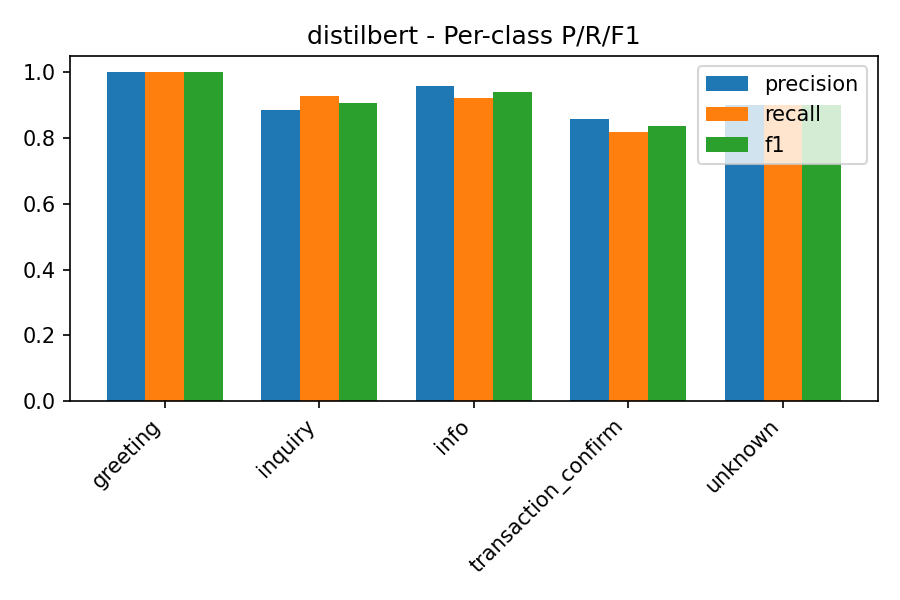
\includegraphics[width=1\textwidth]{../images/distilbert_per_class_prf.png}
\caption{DistilBERT per-class classification report on the held-out test set}
\label{fig:DistilBERT_PerClass}
\end{figure}


\noindent \textbf{Notable finding:} \texttt{transaction\_confirm} shows the lowest
recall (0.82), with 18\% of its samples misclassified as \texttt{inquiry}.  This is
expected: payment-related queries (``I've sent the amount'') share vocabulary with
availability inquiries (``I want to confirm...'').  The agent's dialogue state
validation layer mitigates this---the agent checks conversation state before executing
any booking action, catching misclassified payment messages.

\begin{figure}[h!]
\centering
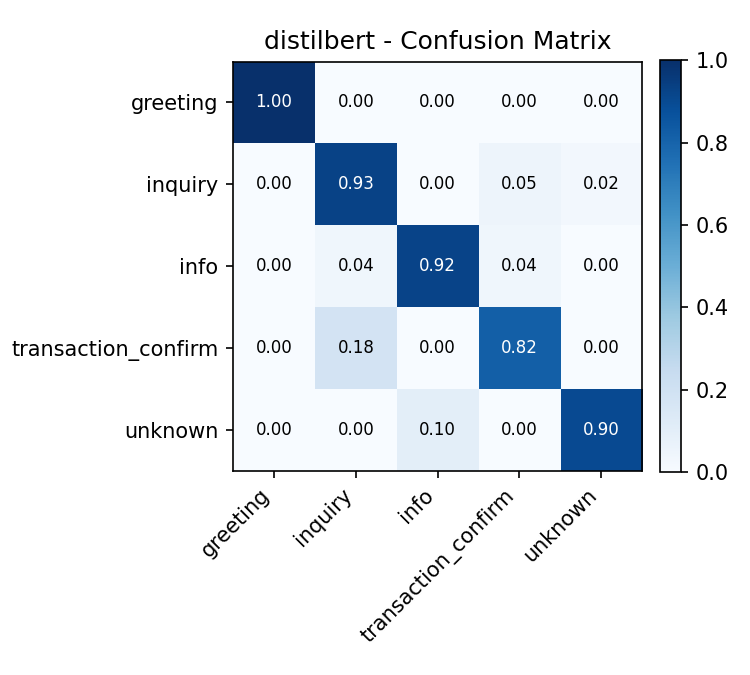
\includegraphics[width=1\textwidth]{../images/distilbert_confusion_matrix.png}
\caption{Confusion matrix for DistilBERT}
\label{fig:DistilBERT_confusion}
\end{figure}
% ─────────────────────────────────────────────────────────────────────────────
\section{Agent Evaluation}
\label{sec:results-agent}

\subsection{Test Case Methodology}

The AI Receptionist was tested on the live deployment against a comprehensive
test case document covering seven categories of agent behaviour. Key results are
showcased below.

\subsection{Test Case Results}

Table~\ref{tab:agent-tests} summarises the results of the key test scenarios.

\begin{table}[H]
\centering
\caption{AI Receptionist agent test case results.}
\label{tab:agent-tests}
\small
\begin{tabularx}{\textwidth}{>{\raggedright\arraybackslash}p{0.10\textwidth}Y Y C{0.08\textwidth}}
\toprule
\textbf{Test ID} & \textbf{Scenario} & \textbf{Expected / Actual Behaviour} & \textbf{Result} \\
\midrule
TC-01
  & Random out-of-scope message (``I want pineapple juice'')
  & Agent declines politely and redirects to booking.
  & \cmark \\[4pt]
TC-02
  & Requested slot unavailable (e.g., Ace Padel 10~PM tonight)
  & Agent offers three nearest alternative slots from same or nearby vendor.
  & \cmark \\[4pt]
TC-03
  & Mid-conversation context switch in Roman Urdu (``padel kal'')
  & Agent correctly parses date reference as tomorrow; time disambiguated via
    follow-up question.
  & \cmark \\[4pt]
TC-04
  & OCR: payment screenshot with incorrect amount (Rs 500 vs required Rs 2000)
  & Agent auto-rejects, informs user of discrepancy, requests corrected screenshot.
    Vendor is not notified.
  & \cmark \\[4pt]
TC-05
  & OCR: unreadable / low-quality image
  & Agent requests a clear screenshot; booking hold maintained.
  & \cmark \\[4pt]
TC-06
  & Successful end-to-end booking flow (English)
  & Booking confirmed, ticket ID \texttt{APD-14} issued, Rs 2000 verified.
  & \cmark \\[4pt]
TC-07
  & Successful end-to-end booking flow (Roman Urdu)
  & Agent handles ``raat'' (night) time reference; booking confirmed in Urdu.
  & \cmark \\[4pt]
TC-08
  & Concurrent booking (OCC): two users request same slot simultaneously
  & Only one booking succeeds; second user receives conflict error and alternatives.
  & \cmark \\[4pt]
TC-09
  & Hold expiry: user does not complete payment within 10 minutes
  & Booking status reverts to AVAILABLE; user notified that hold has expired.
  & \cmark \\[4pt]
TC-10
  & Vendor rejects booking after payment verification
  & Slot released to AVAILABLE; user notified of rejection via WhatsApp.
  & \cmark \\
\bottomrule
\end{tabularx}
\end{table}

\noindent All ten test cases passed on the live deployment.  The agent demonstrated
correct handling of the full booking lifecycle, including error paths (OCR rejection,
slot conflicts, hold expiry, vendor rejection).

% ─────────────────────────────────────────────────────────────────────────────
\section{Discussion}
\label{sec:results-discussion}

\subsection{Key Findings}

\begin{enumerate}
  \item \textbf{Compact models outperform large multilingual models on small
        domain-specific datasets.}  DistilBERT (66M parameters) achieves 90.5\%
        accuracy vs XLM-RoBERTa's (270M parameters) 70.5\%.  Domain-specific
        fine-tuning on 657 utterances contributes more than additional model capacity.

  \item \textbf{The Neuro-Symbolic architecture effectively prevents hallucination.}
        By routing all database mutations through deterministic code nodes, the system
        eliminates the class of errors where agents ``hallucinate'' bookings or bypass
        payment verification.  Zero such failures were observed across 10 structured
        test cases.

  \item \textbf{Roman Urdu code-switching is manageable with targeted augmentation.}
        Despite severe orthographic variation, the DistilBERT model trained on the
        augmented bilingual dataset correctly handled ``padel kal'' (padel tomorrow),
        ``raat'' (night), and other code-switched time references in all test cases.
\end{enumerate}

\subsection{Limitations}

\begin{itemize}
  \item \textbf{Dataset size:} 694 samples is sufficient for a 5-class intent
        classification baseline but insufficient for robust slot extraction across all
        Roman Urdu phonetic variations.  Expanding to 2,000+ samples would improve
        generalisation.

  \item \textbf{Latency on free-tier deployment:} Response times of 38--52 seconds,
        while within the 60-second NFR target, would benefit from caching and a paid
        LLM API endpoint.  Production infrastructure would reduce this to under 10
        seconds.

  \item \textbf{transaction\_confirm confusion:} 18\% misclassification into
        \texttt{inquiry} requires the dialogue state layer as a safety net.  Targeted
        additional training data for this class boundary would address it.

\end{itemize}

%%% Local Variables:
%%% mode: latex
%%% TeX-master: "../report"
%%% End:
